\documentclass[12pt]{article}
\usepackage{graphicx}
\usepackage{eso-pic}
\usepackage{ragged2e}
\usepackage{array}
\renewcommand\thepage{- \arabic{page} -}


\usepackage[utf8]{inputenc}
\usepackage[english]{babel}

\setlength{\parindent}{0em}
\setlength{\parskip}{1em}

%Logo
\newcommand\Highlight{%
	\put(0,150){%
		\parbox[b][\paperheight]{\paperwidth}{%
		\vfill
		\centering
		
\includegraphics[width=\paperwidth, height=10cm]{logo.jpg}%
		\vfill
}}}
%Swirl
\newcommand\Swirl{%
	\put(50,270){%
		\parbox[b][\paperheight]{\paperwidth}{%
		\vfill
		\centering
		
\includegraphics[width=20cm, height=20cm]{background.png}%
		\vfill
}}}
\graphicspath{{../images/}}
\usepackage{graphicx}
\AddToShipoutPicture*{\Highlight}
\AddToShipoutPictureBG{%
	\ifnum\value{page}>1
	\AtPageLowerLeft{\Swirl}%
    \fi
    }%

%Set default path for \input{…} akin to \graphicspath{…}
%https://tex.stackexchange.com/a/79060
\makeatletter
\providecommand*{\input@path}{}
\edef\input@path{{./DataCollection/}{./Introduction/}{./DataStorage/}{./DataPull/}{./StatisticsSubsystem/}{./OverallDescription/}{./UserInterface/}\input@path}% prepend
\makeatother


\begin{document}

{\fontfamily{phv}\selectfont % change phv to get new fonts for whole document
\font\myfont=cmr12 at 20pt

\begin{center}


\begin{minipage}{0.75\linewidth}


\vspace*{250pt}
\title{ \rule{\linewidth}{2pt} \\
\textbf{\normalfont\fontsize{35}{35}\scshape\selectfont IoT HomeCare System}\\
\textbf{\normalfont\fontsize{35}{35}\scshape\selectfont Architectural Design}\\}
\author{
        Hristian Vitrychenko\\
        Nikki Constancon \\
        Juan du Preez\\
        Gregory Austin \\
        Marthinus Richter
}
\date{\today \\ \rule{\linewidth}{2pt}}


\maketitle
\thispagestyle{empty}

\end{minipage}
\end{center}
\pagebreak

\clearpage

\section{Introduction}
\subsection{Purpose}
The purpose of this document is to provide a detailed representation of the ReVA system. This document clearly illustrates and explains the chosen architectural designs of the different parts of the whole system. The system is shown to have different subsystems, and several specific artifacts in the system are explained with the use of diagrams and short summaries in order to make clear how the system is meant to work.
\subsection{Definitions}
\subsection{References}
\subsection{Overview}
The document begins by giving an overall description of the system in the form of a deployment diagram. After that, the separate subsystems are shown and explained in terms of system types and appropriate architectural designs chosen for them. Then, each artifact within the deployment diagram is given its own class diagram and/or other diagrams which clearly expresses the designs and reasons for the chosen designs.

\clearpage
\section{Overall Description}
\subsection{Deployment Diagram}
\begin{center}
\begin{figure}[h]
	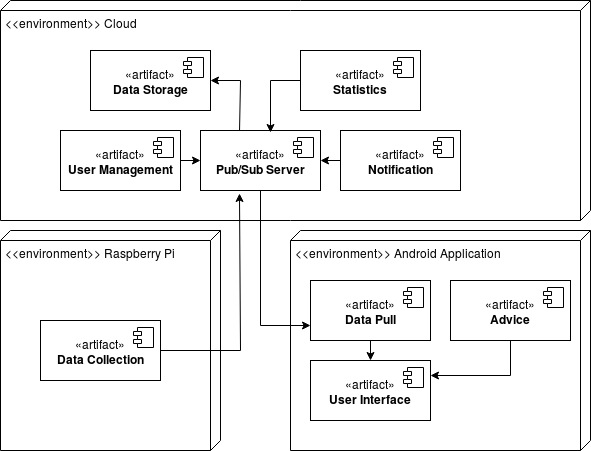
\includegraphics[width=15cm, height=10cm]{OverallDescription/DeploymentDiagram.png}
\end{figure}
\end{center}

\subsection{System and Subsystems}
	The ReVA (Revolutionary Vitality Analyzer) system is the overall system and does not necessarily have a system type, as it is composed of many different subsystems which have their own types and perform different functions as specified in the SRS. If one looks at the system as a whole, it would be an interactive system. This implies that the Android App speaks with and interacts with the server in order to get data from the Raspberry Pi. This is implemented in the Client-Server design. The following subsystems comprise the entire system.

\begin{itemize}
	\item \textbf{Real-Time Subsystem}\\
	This subsystem is responsible for collecting the data, and displaying it real-time on the mobile application. The artifacts which are used are: Data Collection,  Pub/Sub Server, Data Pull, and User Interface. The type of system is a blackboard system since the Data Collection artifact will publish data constantly on the "blackboard" Pub/Sub Server which is situated on the cloud itself. This system is most appropriate because of the constant stream of data, which can be used by subscribers such as the Android application and other modules or artifacts. 
	\item \textbf{Data Storage Subsystem}\\
	This system is responsible for the CRUD functionality of data. It is therefore a persistence framework, and hence a persistence architectural design. The Data Storage artifact subscribes to the Pub/Sub Server, or connects to it by other means, and fills the Cassandra database with data in a format that is ready for research analysis. The persistence is chosen because it fits well with the need for researchers to analyse data, as well as providing an interface for the Statistics module. 
	\item \textbf{History/Statistics Subsystem}\\
	The Data Storage, Statistics, Pub/Sub Server, and User Interface modules work together to provide the user with History and or Statistical data in the form of points on a graph ready to be plotted. This would be an interactive system with a client-server design. The user makes requests via the User Interface to the server which in turn makes use of the Statistics module. The Statistics module gets data from the Data Storage module, and generates the response which the server will return to the user.
	\item \textbf{User Management Subsystem}\\
	All the management of user accounts and sessions, such as registration and logging in/ out, will be handled by the User Management. This is a combination of a client-server and a persistence architecture. Registration etc. requests are originated by the user via the User Interface. This issues a request to the server which consults the User Management module to update a database. 
	\item \textbf{Notification Subsystem}\\
	The notification subsystem is an event-driven type of system. The Notification module is subscribed to the Pub/Sub server, and receives data all the time, analysing it for possible issues. It only reacts to certain events, i.e. in the event of an emergency. This is appropriate because it is completely state-dependent. Reactions and particular alerts are dependent on the states of the data, whether they fall within certain criteria or not.
	\item \textbf{Advice Subsystem}\\
	This subsystem is somewhat of a persistence framework. It is static advice on the app itself, such that the user can know what to do in emergencies. The only modules used are Advice and User Interface.
\end{itemize}

\clearpage
\section{Detailed Artifact Descriptions}
	\subsection{Raspberry Pi Environment}
	
		\subsubsection{Data Collection}
			%diagram
%description
%design patterns
		
	%\subsection{Cloud Server Environment}
	
		%\subsubsection{Pub/Sub Server}
		
	%	\pagebreak
		\subsubsection{Data Storage}
			
			TODO: 
Add inheritance to img
remove addSubscriber option from patientManager


Follows is the description of each manager and the layout of the table that they will manage. It also discusses some of the specialized functions that they will provide.

databaseManager:

	This is the parent class and it established the connection with the database. In the case that the database does 		not exit it will create one. It will do the same for all the tables specified to be in the database.

patientManager:

	This manager will store the identification of the patients on the system. Each patient will be able to obtain a list of all the individuals subscribed to their data, they will also have the ability to remove unwanted subscribers.

	Patient Table:
		(Email, Password, Address, SubscriberPassword, PK(Username), Age, Weight, Height, Reason, SubscriberList) 

	Age: will be an Integer.
	Weight: will be a Double and will be measured in kilograms.
	Height: will be a Double and will be measured in metres
	SubscriberList: will be a set of unique subscriber emails.	
	
	
subscriberManager:

This manager will store all the subscribers or general users. They will be identified by their email address. They will also have the ability to subscribe to patients, in which case the relevant information will be added to both the subscriber's list of patients and the patient's list of subscribers.

	Subscriber Table:
		( PK(Email), Password, Relation, PatientList)
		
		PatientList: will be a set of unique patient usernames.	

patientDataManager:

This manager will have the functionality to retrieve patient data within a time span. The retrieveBetween function will preform this functionality and return a set containing an array of the patient data as well as the max, min and average value obtained during that time span.

	PatientData Table:
		(PK(PatientUsername), PK(DeviceID), PK(TimeStamp), value)
		
		value: can be a double or a set of information.
		
		
		
		
		
		\pagebreak
		\subsubsection{Statistics}
			\begin{center}
\begin{figure}[h]
	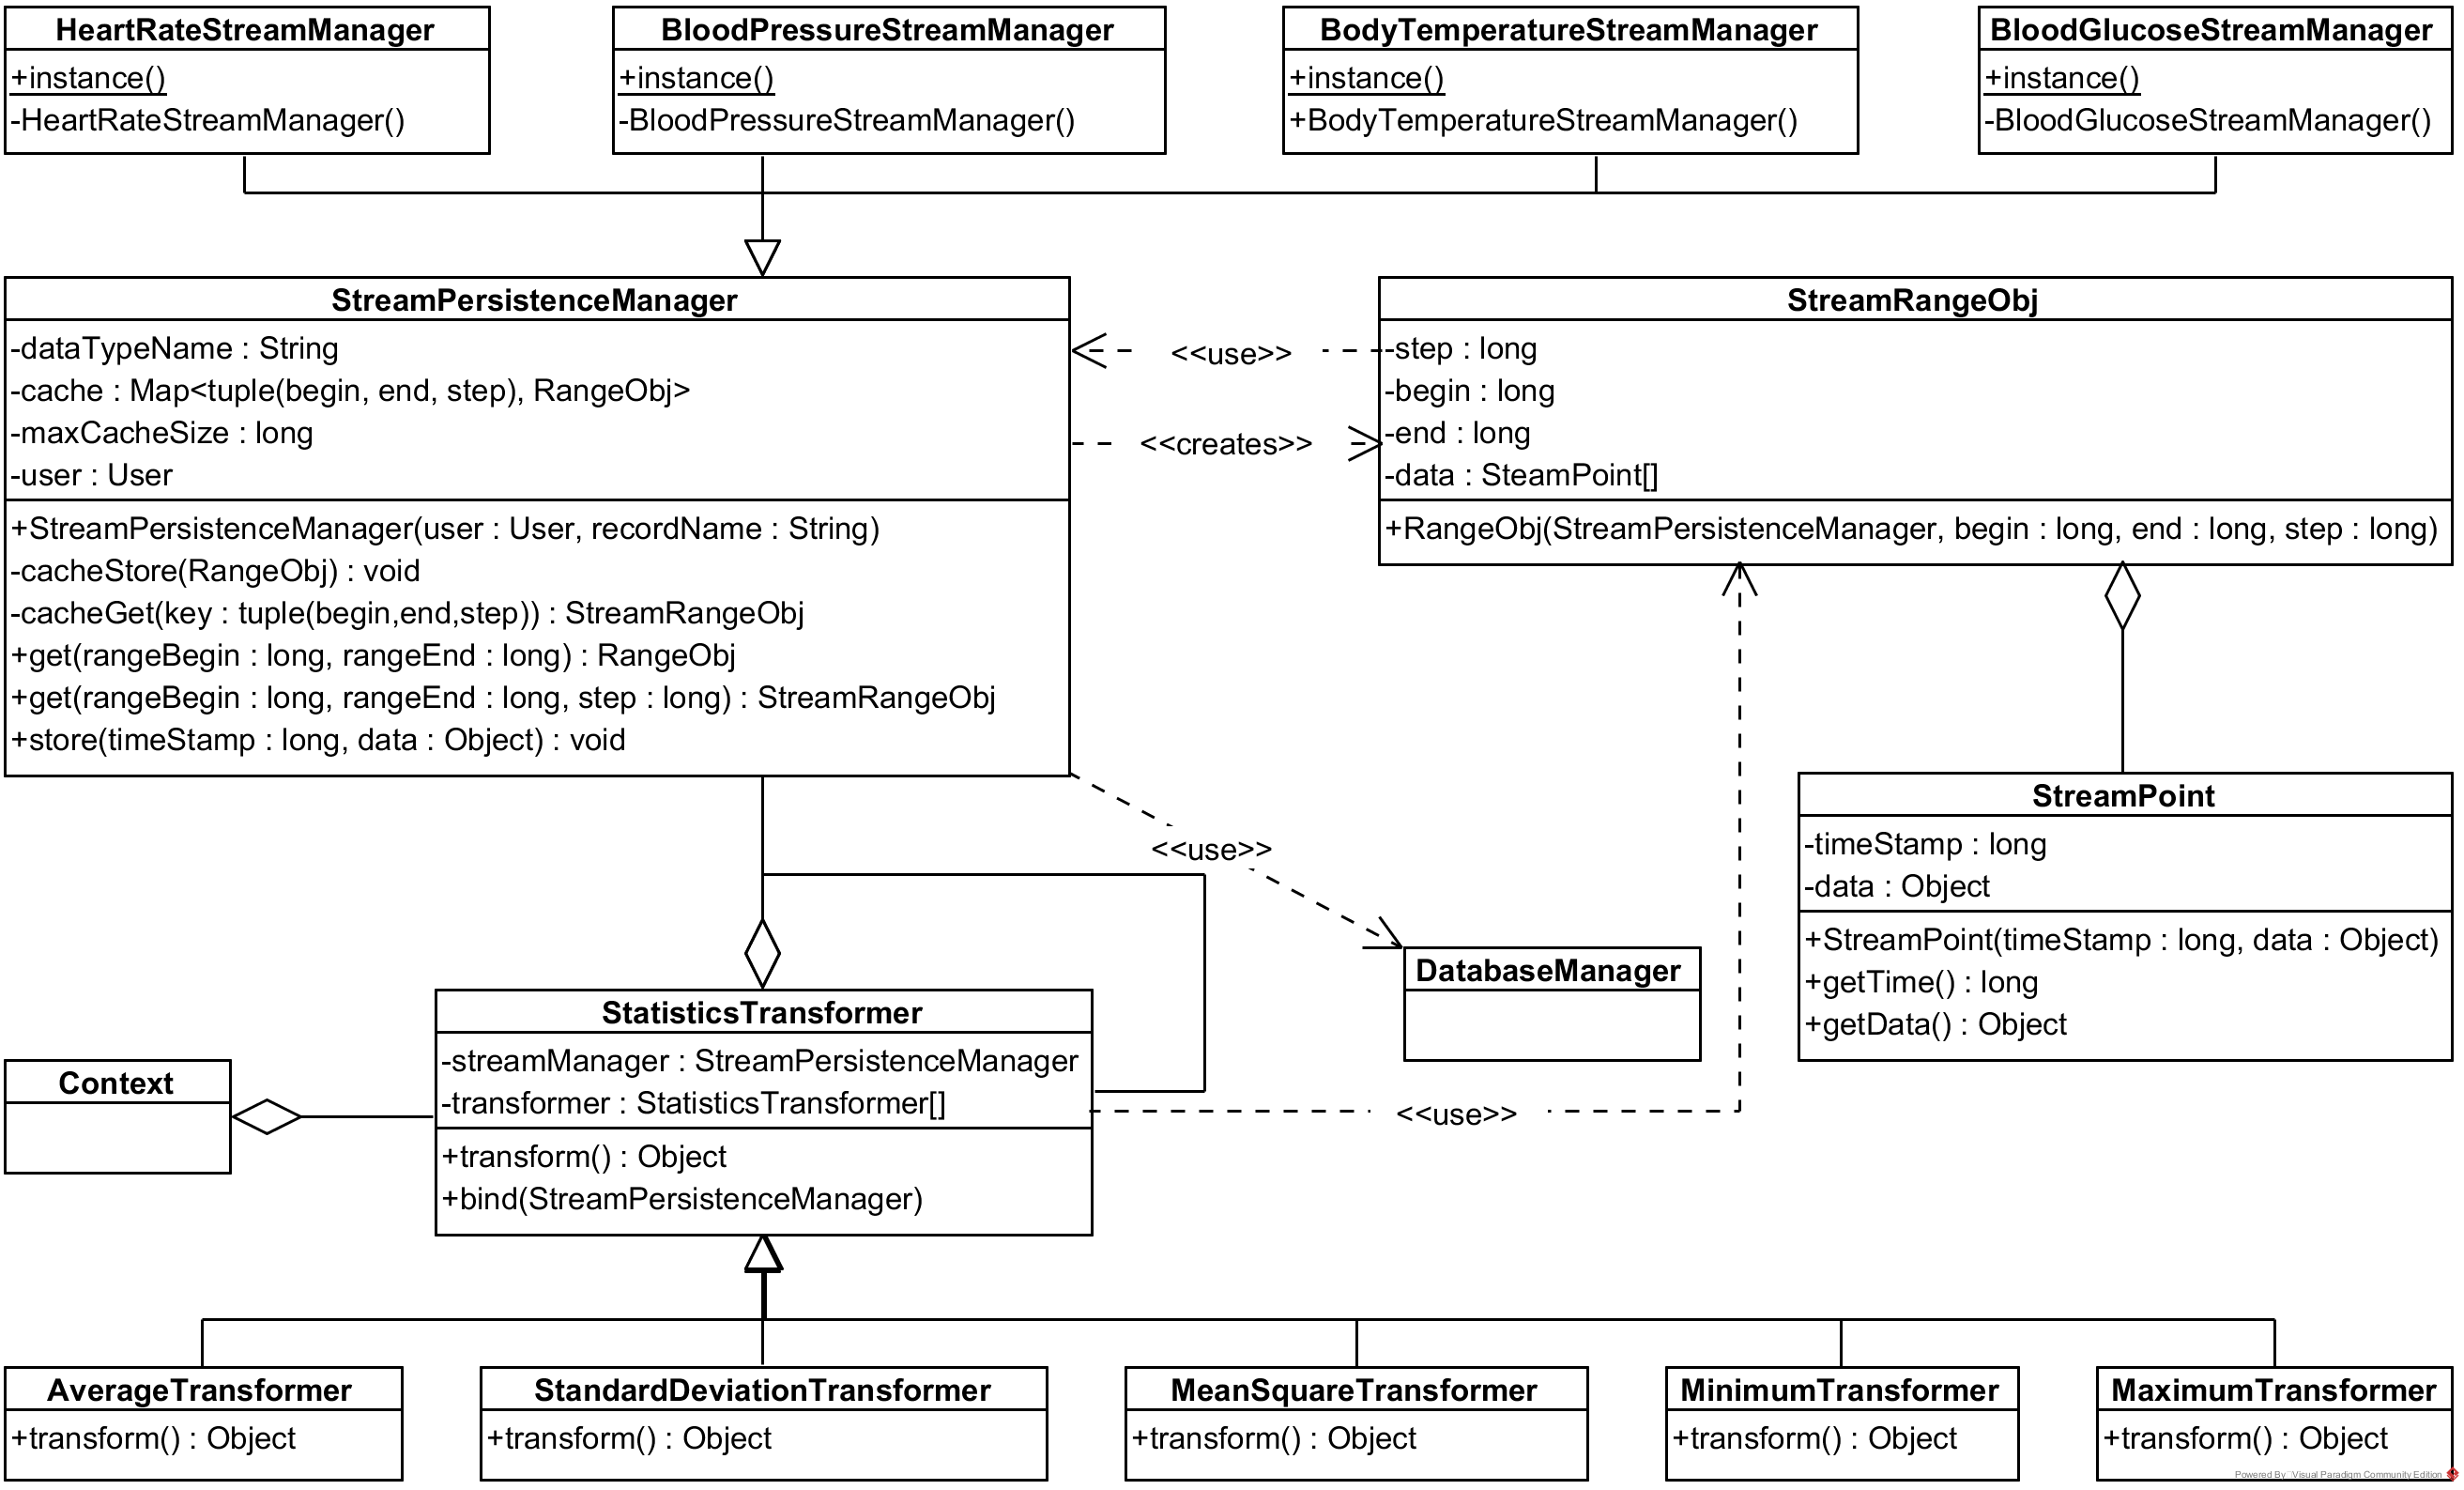
\includegraphics[width=15cm, height=10cm]{StatisticsSubsystem/statisticsClassDiagram.png}
\end{figure}
\end{center}

\begin{itemize}

\item StreamPersistenceManager:\\
This class will assume the responsibility of storing collected data streamed from the RaspberryPI. It will also provide a interface to access said data in a robust manner, such that loose coupling can be achieved with regrades to modules that will transform said data into various representations. A range of collected data may for example be sufficiently queried via the interface.

The stored data will be bound to a specific user and time-stamp. These values will act as primary keys. Each instance of this manager will only manage a single user paired with a specific data representation. These representations may include, but is not limited to: heart rate, body temperature, and blood pressure.

To maximize code reuse, each instance will be initialized with a string that defines what the saved data represents. To minimize conflicts such as data races and overlapping writes to the database, only one instance must be instantiated over the entire process.

\emph{Design Pattern:}
To accommodate code reuse, this class will implement a \textit{Collections Singleton} pattern. A mapping will be made between the tuple composed of the user and data represents, and the related singleton instance.

\item StreamManager:\\
These classes that have \textit{StreamManager} appended to their names will inherit from \textit{StreamPersistenceManager}, and handle a specific data represents. This will logically partition the various representations to increase code readability and maintainability.

\emph{Design Pattern:}
The \textit{Singleton} pattern is simply extended from the supper class.


\item StreamRangeObj:\\
This class will provide robust means to access various data representations. This class will not physically store the stream data, but act as a cache that contains a range of streamed point values. Queries can be satisfied with this class that might need all the streamed data points over a period of time.

The data may be queried with a specified resolution, e.g. only every second value in the series. This will be determined by the step size.


\item StreamPoint:\\
This class will represent each stream data point as a pair, composed of the time-stamp and value.


\item StatisticsTransformer:\\
This is an abstract class that provide the interface to transform various stream data into meaningful statistical values. a specific \textit{StreamPersistenceManager} class may be bound at runtime, so that a sigle instance of this class can potentially compute the statistics for a variety of data representations and an array of different users.

\emph{Design Pattern:}
\begin{itemize}
	\item Strategy: will be used to maximize code reuse
	\item Decorator: will be used to improve modularity and empower the concrete classes to reuse existing \textit{StatisticsTransformer} classes to speed up development.
\end{itemize}


\end{itemize}














		%\subsubsection{Notification}
		
		%\subsubsection{User Management}
		
	\subsection{Android Application Environment}	
	
		\subsubsection{User Interface and Advice}
			\begin{center}
\begin{figure}[h]
	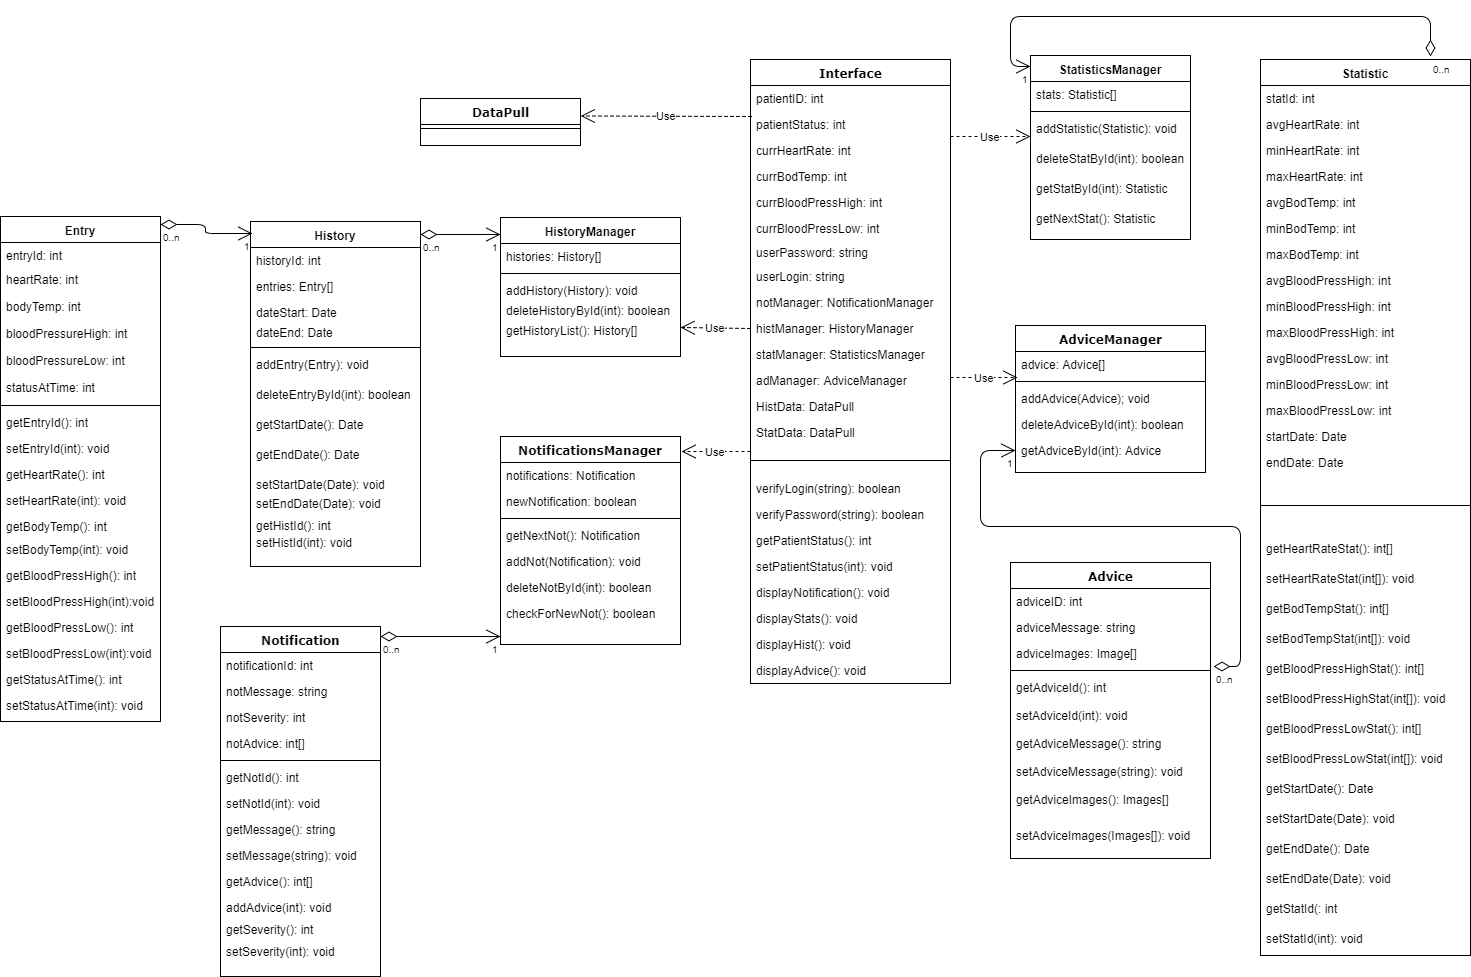
\includegraphics[width=15cm, height=10cm]{UserInterface/Interface.PNG}
\end{figure}
\end{center}

\subsection{Description}
\begin{itemize}
	\item \textbf{DataPull}\\
	This class is not part of the user interface subsystem but serves to represent where data is recieved from i.e. a module from the server. 
	\item \textbf{Interface}\\
	This is the main class of the user Interface subsystem. It serves as the reciever of real-time data and the requester of statistical and historical data. It is meant to keep track of user details as well as register new users. It also keeps track and maintains all managers (NotificationsManager, HistoryManager etc...) and displays their content at the users request. It is the main medium of communication between the application and the server, hence its relation with the DataPull class. 
	\item \textbf{StatisticsManager}\\
	This class acts as a  manager of Statistic class objects. It maintains a list of these objects and provides CRUD (Create, Read, Update, Delete) functionality specifically for statistics. 
	\item \textbf{Statistics}\\
	This class stores statistical data collected from the server from a specified start and end date. It allows for detailed statistics to be recorded and represented by the interface based on the users selection. This class may be vital in noticing outliers in patient health over a certain period of time. 
	\item \textbf{AdviceManager}\\
	This is another manager class but for Advice class objects. It also maintains a list and provides CRUD functionality. 
	\item \textbf{Advice}\\
	This class acts as a container for different advice. Advice is stored in this object in the form of text and is given an ID which is then used to access said advice. Advice may also come with helping images.
  	\item \textbf{HistoryManager}\\
	This is another manager class but for History class objects. It maintains a list of these objects and provides CRUD functionality. 
  	\item \textbf{History}\\
	The History class is a special manager class in that it is a manager class of Entry objects but with a specified start and end date, thus it also acts as a data object. It is built in such a way so as to be able to record historical data through the analysis of the collection of Entry objects which it maintains. It provides CRUD functionality for Entry objects. Through using this class, one is able to plot a graph representing the history of the patient's vitals (done by the Interface class). 
  	\item \textbf{Entry}\\
	Entry is an object class that stores all patient vital's data at a single instance in time. Many Entry objects are used together to establish a history for the patient. 
  	\item \textbf{NotificationsManager}\\
	This is another manager class but for Notification objects. It maintains a list of Notification objects and provides CRUD functionality. This is also a special case manager class in that it stores Notifications based on alerts from the server and not on request from the user. The Interface class would recieve a real time alert from the server and invoke this class to create and store the appropriate notification to be displayed to the user. User may however delete read notifications or choose to keep them as historical references. 
  	\item \textbf{Notification}\\
	This class acts as a holder for appropriate alert messages based on real time patient vital values. It stores a status that indicates how critical the alert is as well as an accompanying message describing the alert. It may also store Advice object ID's for reference and instruction for users to use in situations specific to each individual alert.
\end{itemize}

		\pagebreak		
		\subsubsection{Data Pull}
			%diagram
\begin{center}
\begin{figure}[h]
	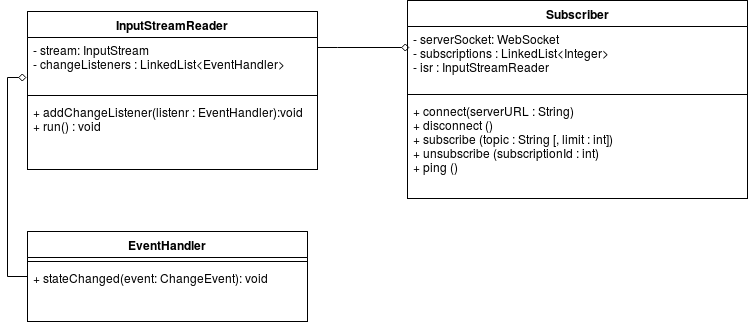
\includegraphics[width=15cm, height=7cm]{DataPull/DataPull.png}
\end{figure}
\end{center}
%description
With the android application we have to communicate with the zetta API platform and get streaming data and other data from the server.
\begin{itemize}
	\item Subscriber:\\
	Subscriber takes care of client-to-server communication using the zetta protocol for each. It makes use of the publish-subscribe model for data streaming. You can connect/disconnect and subscribe/unsubscribe to individual datastreams.

	\item InputStreamReader:\\
	The InputStreamReader is a runnable class so that it can be run by the subscriber class. It takes an inputstream from the server and you can addChangeListeners to cater to each different message the server sends. There is a LinkedList of event handlers that are called with a chain of responsibility.

	\item EventHandler:\\
	An EventHandler can be used by the InputStreamReader so that it can handle each event that the server sends.

\end{itemize}
%design patterns
Chain of Responsibility is used as a design pattern because it suits handling events from the server.

		%\subsubsection{Advice}
		
\clearpage
%\section{Conclusion}
%\input{introduction/design_constraints}
  
\end{document}
